\section{Background Concepts}

In this section, we introduce some fundamental concepts necessary to
understand the overall system design and the class of platforms
targeted by this work.

\subsection{Hybrid Multi-Core Platforms with Programmable Logic}
This work targets a class of embedded platforms that include
traditional full-speed embedded CPUs and programmable logic on the
same chip. This organization naturally defines two macro-domains,
namely the Processing Subsystem (PS) and the Programmable Logic
(PL). The PS encompasses a multi-core processor with a multi-level
cache hierarchy and a main memory (DRAM) controller. We use PS-PL
platforms to refer to this class of SoC for the reminder of this
work. A simplified block diagram for a reference PS-PL organization is
illustrated in Fig.~\ref{fig:PS-PL-diagram}. The figure considers a
platform with four CPUs denoted as $C_0, C_1, C_2$, and $C_3$. 

\begin{figure}[t]
  \centering
  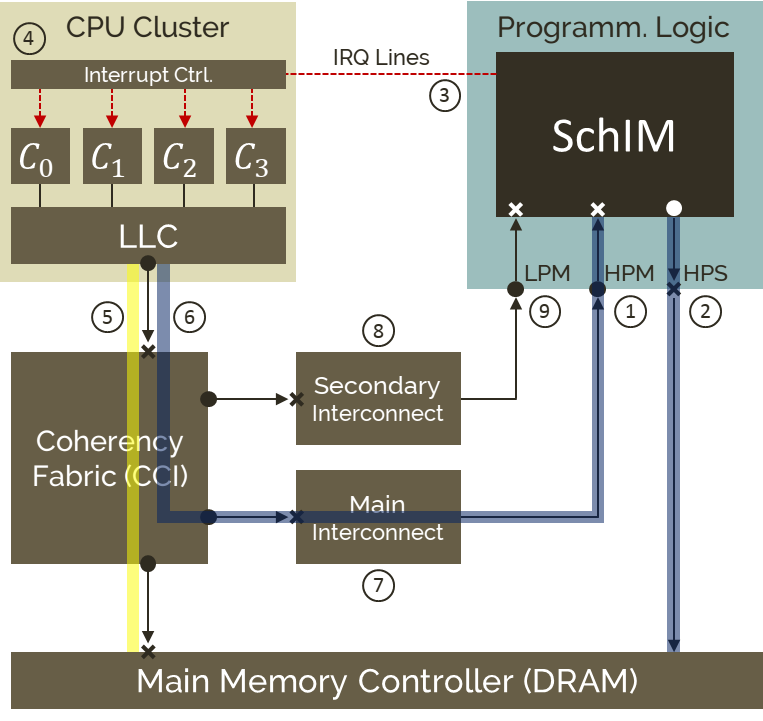
\includegraphics[width=0.9\linewidth]{images/system_blocks.png}
  \caption{PS-PL interconnect block diagram}
  \label{fig:PS-PL-diagram}
\end{figure}

A key feature in PS-PL platforms is the presence of high-performance
communication channels between the two domains. These come in the form
of data exchange interfaces and interrupt lines. Data exchange
channels follow a master-slave paradigm. Specifically,
high-performance masters (HPM, \circledfig{fig:PS-PL-diagram}{1}) and
high-performance slaves (HPS, \circledfig{fig:PS-PL-diagram}{2}) send
and receive transactions to and from the PL,
respectively. Additionally there exist programmable interrupt request
(IRQ) lines (see \circledfig{fig:PS-PL-diagram}{3}) that can be driven
by the PL and are connected to the interrupt controller
(\circledfig{fig:PS-PL-diagram}{4}) inside the PS. As we discuss in
Section~\ref{sec:pl-to-ps-feedback}, the presence of PS-PL interrupt
lines is crucial to build PL-assisted memory traffic regulation.

Note also that there might exist PS-PL data ports that are routed
through a secondary interconnect
(\circledfig{fig:PS-PL-diagram}{8}). These can generally sustain less
throughput compared to HPS ports, hence we refer to them as
low-performance masters (LPM, \circledfig{fig:PS-PL-diagram}{9}). LPM
ports are useful to perform memory-mapped configuration of PL modules.

\subsection{Programmable Logic In-the-Middle}\label{sec:bg_plim}
In this work, we leverage the ability to route main memory traffic
originated by the CPUs through the PL. This technique is known as
Programmable Logic In-the-Middle, or PLIM for short. PLIM was
originally proposed in~\cite{PLIM20}. To understand how PLIM can be
achieved on PS-PL platforms it is important to understand how memory
accesses are routed in such platforms. Any CPU-generated memory access
that results in an LLC miss is routed directly to main memory if its
physical address falls within the aperture, say the address range
$[A,B]$ handled by the DRAM controller. We refer to this as the
\emph{direct route}, depicted in \circledfig{fig:PS-PL-diagram}{5} and
highlighted in yellow.

Conversely, a generic memory access resulting from an LLC cache miss
will be sent on an HPM port if the corresponding physical address
falls within other range, say $[C,D]$. One can then insert (1) a
lightweight layer of virtualization to map all the physical addresses
of a guest OS to the PL, i.e. to fall in the range $[C,D]$; and (2) an
address translator in the PL that re-bases request physical addresses
to access main memory and relays back the data payload to the
requesting CPU(s). In other words, one can find a constant $k$ such
that $C = A + k$. Then, the translator in the PL, upon receiving any
request at address $x \in [C, D]$ will issue a main memory request at
the address $(x - k)$ through the HPS port and provide the response to
the CPU.  The PLIM technique introduces a secondary memory route for
reaching the DRAM, called the \emph{PL loop-back}, or simply
\emph{loop-back}, which is highlighted in blue in
\circledfig{fig:PS-PL-diagram}{6}. Memory transactions on the
loop-back route typically traverse the main interconnect, as depicted
in \circledfig{fig:PS-PL-diagram}{7}. The advantage of PLIM is that
transactions on the loop-back route can be inspected, blocked,
re-routed, and in general managed by custom re-programmable
logic. Importantly, switching from the direct to the loop-back route
can be done dynamically at runtime so that the overhead of PLIM can be
avoided if deemed detrimental for the application under analysis.

Because in this paper we leverage the PLIM approach to perform memory
scheduling, we call our module the \schimL, or \schim for short.

%% The application's memory traffic is intercepted by dispatching them to
%% leave the PS to enter the PL. Intercepted transactions are then
%% forwarded from the PL again toward the memory controller inside the PS
%% using an address translation module. The primary mechanism of PS-PL
%% and PL-PS redirection of a transaction is called the Memory
%% Loop-Back. Loop-Back is done through address bit manipulation of the
%% transaction such that it falls in the range of the target HPM(HPS) for
%% the PS-PL(PL-PS) interception. In this way, the main memory content is
%% accessed, but through a programmable environment, .

%% The underlying mechanism in this work is the ability to intercept
%% memory transactions originated from the processors inside the PS at
%% the PL. APU contains processing cores with private and shared caches
%% alongside a DRAM controller and I/O peripherals. A typical hierarchy
%% for modern embedded SoCs is to fabricate multi-level caches by arming
%% each processor with a private coherent L1 cache and having all
%% processors share a much larger L2 cache. The L2 cache is often also
%% the last-level cache (LLC). Upon a demand for data (or an
%% instruction), the cache is a premier location a processor scans for,
%% surmising for a copy of a required data tobe rapidly accessible, which
%% results in a cache hit. A miss results in the next cache level
%% look-up, and ultimately a miss in LLC provokes access to main memory.

%% While in caches with a write-through policy, the data gets
%% simultaneously written to the main memory as soon as it is updated in
%% the cache; caches with a write-back policy hold the most recent data
%% internally and write it back to the main memory only when it is
%% necessary, i.e., when the cache line is ready to replace. In this
%% sense, these transactions originate from the LLC toward the DRAM
%% \circled{5}. The cache controller is further in charge of determining
%% the replacement policy in the cache. Replacement policy effectively
%% resolves which cache line must be evicted when room for a new line is
%% needed. Conventional replacement policies for associative caches are
%% LRU, PLRU, FIFO, round-robin, and random.

\subsection{Advanced eXtensible Interface (AXI)}
\label{subsec:axi_transaction_scheme}
The vast majority of PS-PL platforms currently available are
ARM-based. This is also the case for the platform we used for our
evaluation, namely the Xilinx Zynq UltraScale+ MPSoC. Thus, we briefly
introduce the communication protocol used of on-chip communication in
ARM-based SoCs, namely the Advanced eXtensible Interface (AXI). The
AXI is a open specification bus protocol~\cite{ARM-AXI} used for
high-bandwidth data exchanges between on-chip subsystems --- such as
cache controllers, memory controllers, DMAs, PL modules. It is also
used in the PS-PL platforms of reference to exchange data on the
aforementioned HPM/HPS ports.

The AXI protocol is based on the master-slave duality. A master AXI
interface can initiate transactions toward a connected slave
interface.  The latter provides a response to master-initiated
requests.  Masters and the slaves communicate with each other through
five different channels named AW (address write), W (write), B (write
acknowledgment), AR (address read) and R (read) as illustrated in
Fig.~\ref{fig:axi_transaction_scheme_figure}.

A write transaction begins with an address phase \circled{1} where the
channel AW is used to transmit the meta-data of the transaction, such
as the destination address, the transaction ID, the cacheability
attributes, the type/length of the burst and so on.  Upon the
completion of this phase, follows the data phase \circled{2} which
consists in the transmission of the data payload to be written through
the W channel.  A successful write transaction is concluded by the
response phase \circled{3} that occurs on the B channel.

The transmission of a read transaction is carried out in a similar
way.  The address phase \circled{1'} is transmitted through the
equivalent AR channel and is directly followed by the data phase
\circled{2'}.  A response initiated by the slave follows where the
read data is transferred over the R channel. The protocol is
asynchronous because different phases of different transactions can
interleave on any AXI bus segment. Hence, multiple outstanding
transactions can be emitted by a single master and the receipt of
out-of-order responses is possible.

\begin{figure}
  \centering
  \begin{tikzpicture}[scale=0.5, every node/.style={scale=0.5}]
    % Module Master
    \draw ( 0.0, 0.0) -- ++( 2.0, 0.0) -- ++( 0.0, 5.25) -- ++( -2.0, 0.0);
    \node[rotate=90] at (0.25, 2.5) {\large MASTER};
    % Module Slave
    \draw (13.0, 0.0) -- ++(-2.0, 0.0) -- ++( 0.0, 5.25) -- ++( 2.0, 0.0);
    \node[rotate=270] at (12.75, 2.5) {\large SLAVE};
    % AW channel
    \node at ( 1.5, 4.50) {AW};
    \draw ( 2.0, 4.25) rectangle ++( 9.0, 0.5);
    \draw ( 5.0, 4.25) rectangle ++( 0.5, 0.5)  node[pos=.5] {A};
    \draw[-{Stealth}] ( 5.5, 4.5) -- ++( 0.5, 0.0);
    \node at ( 11.5, 4.50) {AW};
    \draw[red] ( 6.25, 4.50) circle [radius=0.2] node {1};
    % W channel
    \node at ( 1.5, 3.75) {W};
    \draw ( 2.0, 3.50) rectangle ++( 9.0, 0.5);
    \draw ( 3.0, 3.50) rectangle ++( 0.5, 0.5)  node[pos=.5] {D};
    \draw ( 3.5, 3.50) rectangle ++( 0.5, 0.5)  node[pos=.5] {...};
    \draw ( 4.0, 3.50) rectangle ++( 0.5, 0.5)  node[pos=.5] {D};
    \draw[-{Stealth}] ( 4.5, 3.75) -- ++( 0.5, 0.0);
    \node at ( 11.5, 3.75) {W};
    \draw[red] ( 5.25, 3.75) circle [radius=0.2] node {2};
    % B channel
    \node at ( 1.5, 3.00) {B};
    \draw ( 2.0, 2.75) rectangle ++( 9.0, 0.5);
    \draw ( 9.5, 2.75) rectangle ++( 0.5, 0.5)  node[pos=.5] {B};
    \draw[-{Stealth}] ( 9.5, 3.00) -- ++(-0.5, 0.0);
    \node at ( 11.5, 3.00) {B};
    \draw[red] ( 8.75, 3.00) circle [radius=0.2] node {3};
    % AR channel
    \node at ( 1.5, 1.50) {AR};
    \draw ( 2.0, 1.25) rectangle ++( 9.0, 0.5);
    \draw ( 5.0, 1.25) rectangle ++( 0.5, 0.5)  node[pos=.5] {A};
    \draw[-{Stealth}] ( 5.5, 1.5) -- ++( 0.5, 0.0);
    \node at ( 11.5, 1.50) {AR};
    \draw[red] ( 6.25, 1.50) circle [radius=0.2] node {1'};
    % R channel
    \node at ( 1.5, 0.75) {R};
    \draw ( 2.0, 0.50) rectangle ++( 9.0, 0.5);
    \draw ( 8.0, 0.50) rectangle ++( 0.5, 0.5)  node[pos=.5] {D};
    \draw ( 8.5, 0.50) rectangle ++( 0.5, 0.5)  node[pos=.5] {...};
    \draw ( 9.0, 0.50) rectangle ++( 0.5, 0.5)  node[pos=.5] {D};
    \draw ( 9.5, 0.50) rectangle ++( 0.5, 0.5)  node[pos=.5] {B};
    \draw[-{Stealth}] ( 8.0, 0.75) -- ++(-0.5, 0.0);
    \node at ( 11.5, 0.75) {R};
    \draw[red] ( 7.25, 0.75) circle [radius=0.2] node {2'};
\end{tikzpicture}

  \caption{Caption}
  \label{fig:axi_transaction_scheme_figure}
\end{figure}
